\section{Benchmark NIST-8 "Oscillatory"}
\label{sec:bench-8}

This is a wave function that satisfies the Schr\"{o}dinger's equation model of two
interacting atoms, highly oscillatory near the origin.
The equation solved in this problem is the Helmholtz equation.

\begin{equation} \label{oscillatory}
-\nabla^{2} u - \frac{1}{(\alpha + r)^{4}} u = f
\end{equation}
in the domain $\Omega = (0, 1)^2$, equipped with Dirichlet boundary conditions
given by the exact solution. The exact solution is
$u(x,y) = sin(\frac{1}{\alpha + r})$,
where $r = \sqrt{x^{2} + y^{2}}$, $\alpha = 1 / N \pi$ determines the number of oscillations.
The right-hand side $f$ is calculated by inserting exact solution into (\ref{oscillatory}).
The solution of NIST-8 with $\alpha = 1 / 10 \pi$ is shown in Fig. \ref{fig:sln-nist08}.

\begin{figure}[!ht]
\centering
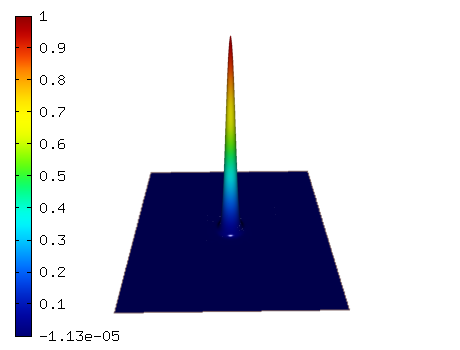
\includegraphics[height=5cm]{nist/nist-8/solution.png}
\caption{The solution to NIST-8 benchmark problem.}
\label{fig:sln-nist08}
\end{figure}

\begin{figure}[!ht]
\centering
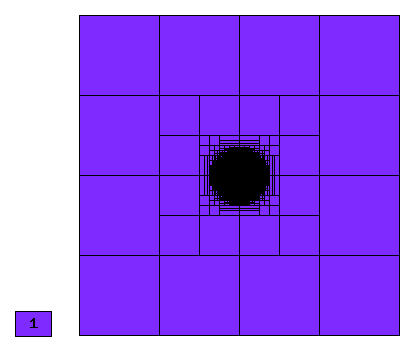
\includegraphics[height=3.7cm]{nist/nist-8/mesh_h1_aniso.png}
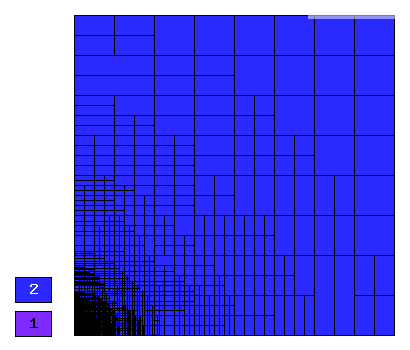
\includegraphics[height=3.7cm]{nist/nist-8/mesh_h2_aniso.png}
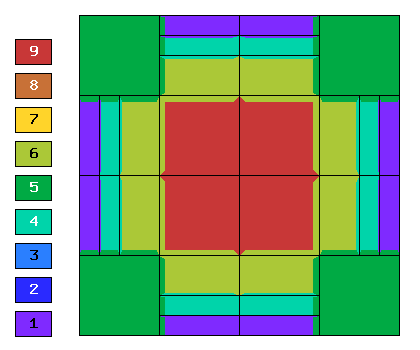
\includegraphics[height=3.7cm]{nist/nist-8/mesh_hp_aniso.png}
\caption{
Final mesh (left) with 55731 DOF and the resulting
relative error estimate in $H^1$-norm of 1.24198 \% for $h$-FEM with linear elements.
Final mesh (middle) with 3413 DOF and the resulting
relative error estimate in $H^1$-norm of 6.64833e-01 1.49585 \% for $h$-FEM with quadratic elements.
Final mesh (right) with 1160 DOF and the resulting
relative error estimate in $H^1$-norm of 9.09848e-02 \% for $hp$-FEM with anisotropic refinements.}
\label{fig:nist-8-hp-aniso}
\end{figure}

%\begin{figure}[!ht]
%\centering
%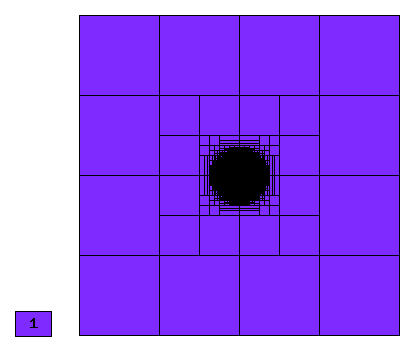
\includegraphics[height=5cm]{nist/nist-8/mesh_h1_aniso.png}\ \
%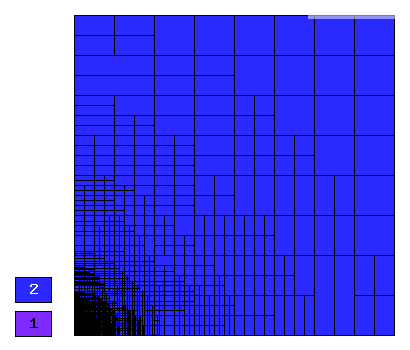
\includegraphics[height=5cm]{nist/nist-8/mesh_h2_aniso.png}
%\caption{Final mesh for $h$-FEM with linear and quadratic elements.}
%\label{fig:nist-8-h-aniso}
%\end{figure}

Figs. \ref{fig:nist-8-conv} compare all
three approaches to automatic adaptivity from the point
of view of DOF and CPU convergence.

\begin{figure}[!ht]
\centering
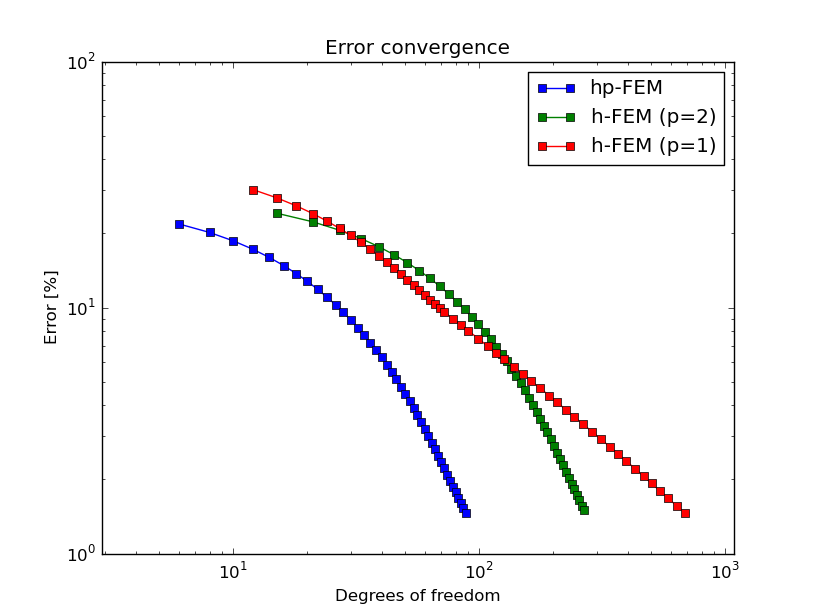
\includegraphics[height=5cm]{nist/nist-8/conv_dof_aniso.png}\ \
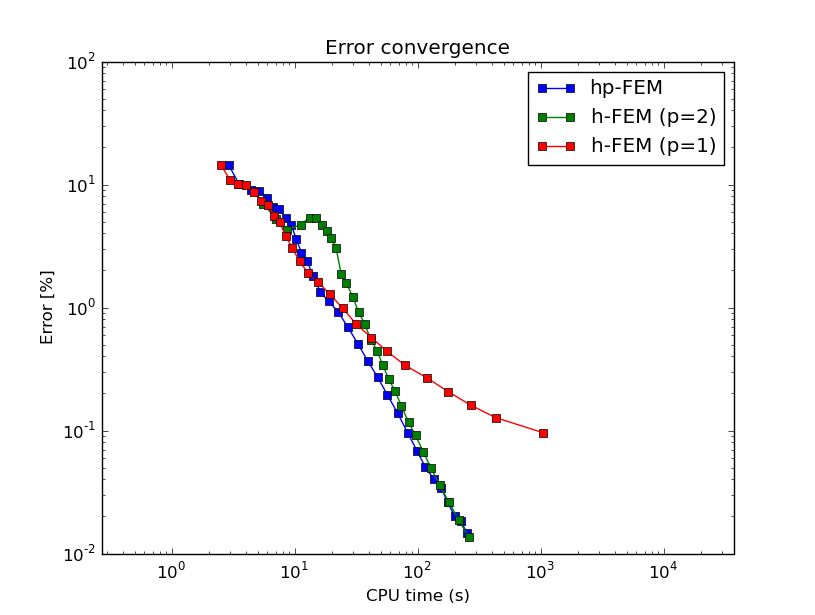
\includegraphics[height=5cm]{nist/nist-8/conv_cpu_aniso.png}
\caption{DOF and CPU time convergence graphs.}
\label{fig:nist-8-conv}
\end{figure}

